\documentclass[twocolumn, openany, oneside, article]{memoir}

\usepackage[style=numeric-comp, backend=biber, bibencoding=utf8]{biblatex}
\usepackage{bm}
\usepackage{amsmath}
\usepackage{amsfonts}
\usepackage{csquotes}
\usepackage[noline, ruled]{algorithm2e}
\usepackage{graphicx}
\usepackage{hyperref}

\bibliography{references}


\DeclareMathOperator{\ifft}{ifft}
\DeclareMathOperator{\fft}{fft}

\title{Scattering representation}
\author{Geert Kapteijns}
\date{\today}

\begin{document}
\maketitle
\pagestyle{simple}

\begin{abstract}

Lorem ipsum dolor sit amet, consectetur adipisicing elit, sed do eiusmod
tempor incididunt ut labore et dolore magna aliqua. Ut enim ad minim veniam,
quis nostrud exercitation ullamco laboris nisi ut aliquip ex ea commodo
consequat. Duis aute irure dolor in reprehenderit in voluptate velit esse
cillum dolore eu fugiat nulla pariatur. Excepteur sint occaecat cupidatat non
proident, sunt in culpa qui officia deserunt mollit anim id est laborum.

\end{abstract}

\chapter{Introduction}

Let me start off by saying this is an informal document meant to make my
research efforts of the last three months accessible. I have made no huge effort
to cite the first paper to establish a concept or even to cite well-established
results at all.

This research is part of a broader effort to use image data to aid radiologists in the process of deciding, in
the earliest possible stage, whether to use intra-arterial therapy (a relatively new endovascular, catheter-based
treatment) to treat ischemic stroke patients.
I have limited my study to classifying brain hemispheres as being affected by stroke or not, thereby finding image features in 3D NCCT scans that are relevant for this decision.

I believe that,
despite popularity and exceptional engineering results in many areas (easily outperforming \enquote{hand-crafted}
algorithms), deep learning is not the best tool for this problem (and I suspect many other problems in the medical
domain), because medical images are high-dimensional, training data is scarce and there is not always a clearly defined
ground truth.

What I have tried here is to use a different approach, namely one where no model is trained for feature extraction, but
which uses an image representation called the scattering transform, that is known to have certain desirable properties,
e.g. it preserves high-frequency information, is translation invariant over a tunable window and stable to deformations.
This image representation may, in association with a simple classifier like an SVM, be used in classification problems.

While detecting which brain hemisphere is affected by stroke is not clinically a very relevant problem (
it can, in most cases, be deducted from the symptoms of the patient) it serves as a test for the scattering representation in 3D, as at
least there is an unequivocal ground truth. Though not done in this work, the learned features may be visualised to aid
radiologists in giving an ASPECTS score or otherwise diagnosing the seriousness of the stroke. It is also possible, if a
good delineation of the ASPECTS regions is available, to directly train a classifier on the scattering representation of
these regions (though expert's opinion on whether a region is affected or not is not unequivocal, making it difficult to
attain super-expert performance).

\chapter{Scattering transform}
I will in the briefest possible way state what the scattering transform is. For details
refer to \cite{anden2014deep, bruna2013invariant}.

A wavelet transform is defined by convolving a $d$-dimensional signal $y(\bm{x})$ with scaled and rotated versions of a
mother wavelet $\psi_{a^j, r}(\bm{x})$, with $j \in \mathbb{Z}$ and rotations $r \in SO(d)$ (rotation group in $d$
dimensions). $d = 3$ in our case, since we are dealing with 3D images. $a = 2$ is common for image analysis. We will
describe in the next section which mother wavelet we use in practice, and how to correctly choose a finite number of
length scales and rotations $r$ (which is not trivial in 3D).

A wavelet of dilation $a^j$ and orientation $r$ looks like
\begin{equation}
  \psi_{a^j, r}(\bm{x}) = a^{-dj} \psi(a^{-j}r\bm{x})
\end{equation}
where the normalisation $a^{-dj}$ is chosen such that the energy of the mother wavelet is
conserved
\begin{equation}
  \int_{\mathbb{R}^d} d\bm{x} | \psi_{a^j, r}(\bm{x}) | = \int_{\mathbb{R}^d} d\bm{x} | \psi(\bm{x}) |.
\end{equation}
Translationally invariant coefficients (called scattering coefficients) of $y(\bm{x})$ that are stable to small deformations are obtained by taking the modulus and taking a spatial average:
\begin{equation}
    \left\| y \star \psi_{a^j, r} \right\|_{1} = \int d\bm{x} |y \star \psi_{a^j, r}|.
\end{equation}
The signals $|y \star \psi_{a^j, r}|$ are themselves unstable, and in averaging (or equivalently, removing all non-zero
frequencies) of $|y \star \psi_{a^j, r}|$ information is lost. To remedy this, we can perform a second wavelet
transform on all first-order transforms, yielding second-order scattering coefficients
\begin{equation}
  \left\| |y \star \psi_{a^{j_1}, r_1}| \star \psi_{a^{j_2}, r_2} \right\| = \int d\bm{x} | |y \star \psi_{a^{j_1}, r_1}| \star \psi_{a^{j_2}, r_2} |
\end{equation}
for all $j_1, j_2, r_1, r_2$. One can keep iterating this transform to recover more lost information in the form of
higher-order coefficients, but in practice two layers is sufficient for most tasks (luckily so, because the
computational resources required scales exponentially in the number of layers).

To make notation easier, we define $\lambda = (j, r)$ and
\begin{equation}
  U[\lambda_1, \dots \lambda_m]y = \left| \left| \left| y \star \psi_{\lambda_1} \right| \star \psi_{\lambda_2} \right|
  \dots \psi_{\lambda_m} \right|
\end{equation}
i.e. an unaveraged signal at the $m$th layer. The scattering coefficients
at the $m$th layer are then written
\begin{equation}
  \left\{ \bar{S}y(\lambda_1, \dots \lambda_m) = \int d\bm{x} U[p]y \right\}_{\lambda_i \in \Lambda}
\end{equation}

In practice it is often better not to average over the entire signals $U[p]$ (where we write $p = \lambda_1, \dots
\lambda_m$ a \emph{path}), but compute coefficients that are approximately translation invariant over lengths $a^J$.
This is achieved by computing the wavelet transforms only at scales $j \leq J$ and averaging with a low-pass (blurring) filter (in
practice a Gaussian) of support $a^J$, denoted by $\phi_{a^J}$
\begin{equation}
  S[p]y(\bm{x}) = (U[p] \star \phi_{a^J})(\bm{x}).
\end{equation}
$\left\{ S[\lambda_1, \dots, \lambda_m] \right\}_{\lambda_i \in \Lambda}$ are called the windowed scattering
coefficients at layer $m$. The correct maximum length scale $a^J$ should be chosen based on knowledge about the input
data or by cross-validation.

\chapter{Implementation details}
What follows are some considerations for choosing the mother wavelet and
rotations $r$.

\section{Construction of the mother wavelet}

For the scattering representation to be stable to additive noise and contain all
high frequency information, it must satisfy the Littlewood-Paley condition
\begin{equation}\label{eq:lp_condition}
  (1 - \epsilon) \leq A(\bm{\omega}) \leq 1 \qquad \forall \bm{\omega} \in \mathbb{R}^d
\end{equation}
with
\begin{equation}
  A(\bm{\omega}) = \left| \hat{\phi}_{a^J}(\bm{\omega}) \right|^2 + \frac{1}{2} \sum_{j \leq J} \sum_{r \in R}
  \left( \left| \hat{\psi}_{a^j, r}(\bm{\omega}) \right|^2 + \left| \hat{\psi}_{a^j, r}(\bm{-\omega}) \right|^2 \right)
\end{equation}
and $\epsilon$ small. Since the low-pass filter $\phi_{a^J}$ is normalized ($\int d\bm{x} \phi_{a^J}(\bm{x}) = 0$ or
equivalently $\hat{\phi}_{a^J}(\omega = 0) = 1$), the above condition implies
\begin{equation}\label{eq:averages_to_zero} \hat{\psi}_{a^j, r}(0) = 0 \end{equation} or equivalently: all wavelets
should average to zero.
Furthermore, if we define a mother wavelet, called the Morlet wavelet, as follows
\begin{equation}
  \psi(\bm{x}) = \mathcal{N} g_{\sigma}(\bm{x})\left( e^{i \xi \bm{x}} - \kappa_{\sigma} \right)
\end{equation}
where $g(\bm{x})_{\sigma}$ is a Gaussian and $\kappa_{\sigma} \ll 1$ has to be chosen to satisfy
\autoref{eq:averages_to_zero}, it will have the property that its Fourier transform is real, hence that if the input
signal $y$ is real, $U[j, r]y = U[j, -r]y$, allowing us to only consider positive rotations.

Instead of labeling a wavelet by its standard deviation in the spatial domain $\sigma$, it is in this case
more insightful to label it by its bandwidth $b$ in the Fourier domain, defined by
\begin{equation}
  \hat{g}_{\sigma}\left(\pm \left(\frac{b}{2}, 0, 0 \right) \right) = \exp \left( -\frac{1}{2}\sigma^2 \left(\frac{b}{2}\right)^2 \right) = \frac{1}{\sqrt{2}}
\end{equation}
leading to
\begin{equation}
  b^2 = \frac{4 \ln 2}{\sigma^2}.
\end{equation}

The Fourier transform of the Morlet is
\begin{equation}
  \hat{\psi}(\bm{\omega}) = \mathcal{N} \left( \hat{g}_{\sigma}(\bm{\omega} - \bm{\xi}) -
  \kappa_{\sigma}\hat{g}_{\sigma}(\bm{\omega}) \right) .
\end{equation}
It is, apart from the small factor $\kappa_{\sigma}$, centered at
$\bm{\xi} = (\xi, 0, 0)$ with bandwidth $b$.
The requirement $\hat{\psi}(\bm{0}) = 0$ leads to
\begin{equation}
  \kappa_{\sigma} = \frac{\hat{g}_{\sigma}(-\bm{\xi})}{\hat{g}_{\sigma}(\bm{0})}.
\end{equation}
The dilated and scaled wavelet becomes in the Fourier domain
\begin{equation}
  \hat{\psi}_{a^j, r}(\bm{\omega}) = a^{-dj} \mathcal{N} \left( \hat{g}_{\sigma}(a^j r^{-1} \bm{\omega} - \bm{\xi}) - \kappa_{\sigma}\hat{g}_{\sigma}(a^j r^{-1} \bm{\omega}) \right)
\end{equation}
so that it is (apart from the small corrective term $\kappa_{\sigma}$) centered at frequency $\bm{\omega_c} =
a^{-j}r\bm{\xi}$ with bandwidth $b_{a^j} = a^{-j}b$. Note that the corrective factor $\kappa_{\sigma}$ is invariant
under dilation and rotation.

We choose the normalisation factor of the mother wavelet $\mathcal{N}$,
in order to be able satisfy \autoref{eq:lp_condition}, as the inverse of the maximum of the \enquote{raw} Littlewood-Paley
sum (which excludes the contribution of the low-pass filter)
\begin{equation}
  \mathcal{N}^{-1} = \max_{\bm{\omega}} \frac{1}{2} \sum_{j \leq J} \sum_{r \in R}
  \left( \left| \hat{\psi}_{a^j, r}(\bm{\omega}) \right|^2 + \left| \hat{\psi}_{a^j, r}(\bm{-\omega}) \right|^2
  \right).
\end{equation}


\section{Discretizing $SO(3)$}

We still need to specify which rotations we will use to build our filter bank, and, consequently, what the correct
values of $\xi$ and $b$ are to satisfy \autoref{eq:lp_condition}. Thanks to the Morlet wavelet having a real
Fourier transform and our CT images being real, we only have to choose a finite number of positive rotations so that our
scaled and rotated wavelets cover (are non-zero) on as much of the frequencies
\begin{equation}\label{eq:positive_halfspace}
(\omega_x, \omega_y, \omega_z) \qquad 0 < \omega_x < \pi, -\pi < \omega_y, \omega_z < \pi
\end{equation}
as possible, where $\pi$ is the Nyquist frequency in radians (equal to $N/2$ for an $N \times N \times N$ image). In practice, we can
impose the additional constraint
\begin{equation}\label{eq:freq_ball}
    \omega_{x}^2 + \omega_{y}^2 + \omega_{z}^2 \leq \pi^2
\end{equation}
since we don't care so much about the highest possible frequencies in the signal (they are very small anyway).

A scaled and rotated wavelet has Fourier support around $\bm{\omega_c} = a^{-j}r\bm{\xi}$ with bandwidth $b_{a^j} =
a^{-j}b$. Hence, because $\bm{\xi} \propto (1, 0, 0)$ and we essentially want to cover the half-ball described by
\autoref{eq:positive_halfspace} and \autoref{eq:freq_ball}, we should choose our rotations $r$ such that they map the
unit vector $(1, 0, 0)$ onto $n$ points on the hemisphere with north pole $(1, 0, 0)$ such that the pairwise distance in
$\mathbb{R}^3$ is maximal (i.e. they are \enquote{evenly spread out} across the hemisphere).

Placing our points on the corners of a platonic solid is ideal, but only works for at most 10 points (the regular
dodecahedron). For a solution for general $n$, I have used the Fibonacci lattice, which distributes $n$ points to
maximize their distance \emph{along the sphere} in an approximately optimal way, but this should be a good approximation
to the problem at hand when to number of points is large.


\section{Choosing $\xi$ and $b$}


\chapter{Experiment on NCCT baseline scans}

I used NCCT data from the MRCLEAN registry. To obtain 3D pictures of the brain
hemispheres, I performed a rigid transform onto an \enquote{atlas} (a perfectly
aligned model image) using the Elastix library \cite{elastix}, then used a
region-growing algorithm to select only the pixels that belonged to brain
tissue, then separated the hemisperes by cutting over the y-axis and finally
resampled the image to dimensions $(128, 256, 128)$, to avoid having to zero-pad
before doing the scattering transform.

I manually checked the center slices of the registered images and removed images
for which rigid registration failed for some reason. I also removed patients
with signs of earlier stroke. In this way, I selected 150 brain scans, yielding
a dataset with 150 samples in each class. See \autoref{fig:input_hemisphere} for
an example of an input affected hemisphere.

\begin{figure}
  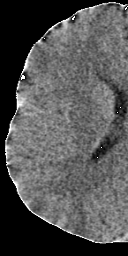
\includegraphics[width=0.6\linewidth]{hemisphere_slice}
  \caption{Axial slice of an input image of an affected brain.}
  \label{fig:input_hemisphere}
\end{figure}

\section{Scattering parameters}

For the classification experiment, I used $\xi = \frac{4\pi}{5}$ and $\sigma =
0.0129$ for the mother wavelet, and constructed a filter bank for $J = 4$ and
using rotations that map the vector $(1, 0, 0)$ onto 20 upper-hemisphere points
of the Fibonacci lattice. This satisfies the Littlewood-Paley condition
\autoref{eq:lp_condition} with $\epsilon = 0.92$ and an average deficiency
$\epsilon_{\mathrm{avg}} = 0.29$. This is a lot worse than \cite{bruna2013scattering}
obtains for experiments in 2D, but it is to me unclear what can be done to obtain a better coverage
of Fourier space in 3D.

\section{Support vector machine classifier}

I selected the SVM that had the highest precision on 80\% of the dataset (with
equal number of samples per class) with five-fold cross validation, from a set of linear SVMs with
regularisation paramater $C \in \{1, 10, 100, 1000\}$ and Gaussian radial basis function kernel SVMS with
the same $C$ and $\gamma \in \{ 10^{-3}, 10^{-4}, 10^{-5}, 10^{-6} \}$. The Gaussian kernel SVM with $C = 10$ and $\gamma = 10^{-5}$
performed the best with 80\% precision on the training set. It obtained a \textbf{73\% precision} on the remaining 20\% of the dataset.

\chapter{Discussion}


\appendix

\chapter{Fast implementation}

In this appendix, I will outline some straightforward steps to speed up the
numerical implementation of the scattering transform, which is especially
necessary in 3D.

Most of the energy is contained in the first two layers of the scattering
transform, and especially in the subset of propagated signals with $j_1 < j_2$
\cite{bruna2013invariant, mallat2012group} (this is a typo in \cite{bruna2013}
under the header \enquote{Fast Scattering Computations}, which says $j_1 \leq
j_2$). I therefore only compute these paths in the implementation.
Furthermore, signals that have been convolved with a filter at scale $a^j$,
contain mostly frequencies below $\pi a^{-j}$, so can be safely downsampled by a factor $a^j$.
(This also is true for the scattering coefficients $U[p] \star \phi_{a^J}$, which can be downsampled by a factor
$a^J$ at all layers.)

To implement the actual convolutions, it is of vital importance to perform them
as a product in the Fourier domain (per the convolution theorem). It is therefore efficient to contstruct
the filter bank in the Fourier domain and to keep downsampled versions in memory. Because we only
consider the subset of paths with $j_1 < j_2$, we need a wavelet of length scale $a^j$ downsampled at
scales $a, a^{2}, \dots a^{j-1}$. See \autoref{algorithm:filterbank}.

For pseudocode for the scattering transform, see \cite{bruna2013invariant}.
To compute signals $|y \star \psi_{a^j, r}|$, it is more efficient to downsample in the Fourier domain,
since that saves time in the inverse Fourier transformation, see \autoref{algorithm:scattering_operator}.
The equivalent of downsampling a spatial signal by a factor $D$, i.e.
\begin{equation}
  x_D[n] = x[Dn]
\end{equation}
corresponds in the Fourier domain to
\begin{equation}
  X_D[\omega] = \frac{1}{D}\sum_{k=0}^{D-1}X(\frac{\omega - 2 \pi k}{D}).
\end{equation}
Note that both the construction of the filter bank and the scattering operations can be sped up
by performing them with a GPU.

A final thing that might be attempted is to speed up elementwise multiplication
in the Fourier domain by cropping the filters $\hat{\psi}_{a^j, r}$, see \cite{ifftmultiply}
for a code example in 1D.

\begin{algorithm}
\For{$0 \leq j \leq J$ and $r \in R$}{
  construct $\hat{\psi}_{a^j, r}(\bm{\omega})$\;
  \For{$j' \in \{1, \dots, j-1\}$}{
    downsample $\hat{\psi}_{a^j, r}(\bm{\omega})$ by factor $a^{j'}$\;
  }
}
construct $\hat{\phi}_{a^J}(\bm{\omega})$\;
\For{$j \in \{1, \dots, J\}$}{
  downsample $\hat{\phi}_{a^J}(\bm{\omega})$ by factor $a^j$\;
}
\caption{Constructing the wavelet filter bank.}\label{algorithm:filterbank}
\end{algorithm}

\begin{algorithm}
  \SetKwInOut{Input}{Input}
  \SetKwInOut{Output}{Output}
  \Input{Fourier transforms $\hat{y}$ and $\hat{\psi}_{a^j, r}$.}
  Compute elementwise product $\hat{y} \cdot \hat{\psi}_{a^j, r}$\;
  Downsample $\hat{y} \cdot \hat{\psi}_{a^j, r}$ by factor $a^j$\;
  $y \star \psi_{a^j, r} \leftarrow \ifft(\hat{y} \cdot \hat{\psi}_{a^j, r})$\;
  Compute $|y \star \psi_{a^j, r}|$\;
  Compute $\fft(|y \star \psi_{a^j, r}|)$ for extracting scattering coefficients and next layer's transform\;
  \caption{Computing $|y \star \psi_{a^j, r}|$.}\label{algorithm:scattering_operator}
\end{algorithm}






\printbibliography

\end{document}

% I downsample in the Fourier domain by a factor $2^j$ by simply setting to zero all frequencies
% outside the range $[-\frac{\pi}{2^j}, \frac{\pi}{2^j}]$ in each dimension. This ideal low-pass filter corresponds to a
% convolution with a normalized sinc-filter in the spatial domain.
